\documentclass[11pt]{article}
% Figures generated by scripts/export_paper_assets.py
% Preamble for the agency paper
\usepackage[T1]{fontenc}
\usepackage{lmodern}
\usepackage[margin=1in]{geometry}
\usepackage[utf8]{inputenc}
\usepackage{microtype}
\usepackage{amsmath,amssymb,mathtools}
\usepackage{graphicx}
\usepackage{booktabs}
\usepackage{tabularx}
\usepackage[font=small,labelfont=bf]{caption}
\usepackage{tikz}
\usetikzlibrary{arrows.meta,positioning,calc}
\usepackage{xcolor}
\usepackage{fancyhdr}
\usepackage{hyperref}
\usepackage{xurl}
\hypersetup{
  colorlinks=true,
  linkcolor=blue!70!black,
  citecolor=green!50!black,
  urlcolor=blue!80!black,
  bookmarksnumbered=true,
  pdfauthor={Ioannis Tsiokos},
  pdftitle={To Throw a Stone with Six Birds: On Agents and Agenthood}
}
\usepackage{enumitem}
\usepackage{natbib}
\usepackage[capitalise,noabbrev]{cleveref}
\usepackage{orcidlink}

\newcommand{\SBT}{Six Birds Theory}
\newcommand{\Emp}{\mathrm{Emp}}
\newcommand{\K}{\mathcal{K}}
\newcommand{\Alpha}{\mathcal{A}}
\newcommand{\Def}{\mathrm{Def}}
\newcommand{\Post}{\mathrm{Post}}
\newcommand{\Safe}{\mathrm{Safe}}
\newcommand{\Afeas}{A_{\mathrm{feas}}}
\DeclareUnicodeCharacter{03B1}{\ensuremath{\alpha}}
\DeclareUnicodeCharacter{2200}{\ensuremath{\forall}}
\DeclareUnicodeCharacter{2203}{\ensuremath{\exists}}
\DeclareUnicodeCharacter{2192}{\ensuremath{\to}}
\DeclareUnicodeCharacter{2286}{\ensuremath{\subseteq}}
\DeclareUnicodeCharacter{2227}{\ensuremath{\wedge}}

\newcommand{\lean}[1]{\path{#1}}


% Affiliation helper (HAL-compatible author block).
\makeatletter
\newcommand{\affiliation}[1]{\gdef\@affiliation{#1}}
\newcommand{\printaffiliation}{\begin{center}\small \@affiliation\end{center}}
\makeatother

\title{To Throw a Stone with Six Birds: On Agents and Agenthood}
\author{Ioannis Tsiokos\,\orcidlink{0009-0009-7659-5964}}
\affiliation{}
\date{31 January 2026\\[4pt]{\small Version 3 (6 October 2026) \quad$\cdot$\quad DOI: \href{https://doi.org/10.5281/zenodo.23184176}{10.5281/zenodo.23184176}}}

\fancypagestyle{firstpage}{%
  \fancyhf{}
  \fancyfoot[C]{\scriptsize Automorph Inc., Wilmington, DE, USA \quad \texttt{ioannis@automorph.io} \quad DOI: \href{https://doi.org/10.5281/zenodo.23184176}{10.5281/zenodo.23184176} \quad \textcopyright\ 2026 \quad CC-BY 4.0 \quad Preprint --- not peer reviewed.}
  \renewcommand{\headrulewidth}{0pt}
  \renewcommand{\footrulewidth}{0pt}
}

\begin{document}
\maketitle
\thispagestyle{firstpage}
\printaffiliation

\begin{abstract}
What does it take for a system to have choices that make a difference? We study this question in finite controlled Markov kernels, without assuming goals, utilities, or an inner agent. Following Six Birds Theory (SBT) \citep{six_birds_theory}, we treat an agent as a \emph{theory object}: a package that is maintained inside an induced description of the system and that has a budgeted interface to the rest of the world. This lets us separate \emph{agenthood}, the existence and persistence of such a package, from \emph{agency}, the ability of its interface choices to change what happens outside. Three computable measures make the distinction concrete: the viability kernel (the largest set of safe states in which every state has an affordable action whose possible successors all remain in the set), feasible empowerment (the channel capacity from affordable action sequences to a later outside variable), and the idempotence defect of a coarse-grained packaging map. Two null tests guard against false positives: a single-action system has zero empowerment, and an external schedule mistaken for an action yields a spurious 1~bit. In a small ring world with switchable mechanisms we then obtain three controlled comparisons. With funded preventive repair, the packaging defect at a full phase cycle falls from 1 to 0 and the set of states that can be kept coherent grows from empty to 16; controls show that a zero defect alone does not identify maintenance. A phase-dependent step leaves one-step empowerment unchanged but raises the sampled median at two steps from 1.21 to 1.72~bits. Reducing slip raises median empowerment from 0.84 to 1.37~bits. A Lean~4 development proves that the viability iteration reaches the greatest safe controlled-invariant set after at most as many strict removals as there are safe states. All results are finite witnesses produced by deterministic, audited scripts.
\end{abstract}
\noindent\textbf{keywords:} agency; agenthood; viability kernel; controlled invariance; empowerment; channel capacity; Markov decision processes; reproducible artifacts

% \tableofcontents

\section{Introduction}
\label{sec:introduction}

\subsection{To throw a stone}
To throw a stone is to make a reliable difference to the world: after the throw, the world is measurably different from how it would otherwise have been. The sentence sounds trivial until one asks what must already be in place for it to mean anything. In a substrate of micro-interactions, where is the throw? Which degrees of freedom are the thrower, which the stone, and which the outside world? When does a subsystem have \emph{choices}, rather than simply being pushed around?

This paper treats agency as something \emph{induced} rather than assumed. We do not start from goals, intentions, or preferences. We start from a finite stochastic system and ask two questions: when does a stable, budgeted subsystem exist at all, and when do its feasible choices change the distribution of outside futures? The stone is a reminder that the second question is about counterfactual difference-making under constraints: there should be at least two affordable ways of acting that lead to distinguishable outcomes.

\subsection{From objects to agents in Six Birds Theory}
In \SBT\ \citep{six_birds_theory}, macroscopic objects are not primitives. The theory proposes six emergence mechanisms, the ``six birds'', that together make stable macroscopic descriptions possible: operator rewriting, constraints on what is feasible, protocol cycles, identity and staging, closure, and resource accounting. On this view an object is a stabilised package: a description that persists long enough to be treated as a thing with a boundary.

If objects are induced, agents should be too. A companion paper on life \citep{six_birds_life} treats living systems as maintained, self-accounting closures rather than as a list of biological exceptions. Here we ask the parallel question for agency: what must be in place before something like an action exists, and once it exists, what does it mean for that action to be a cause?

\subsection{Agenthood and agency}
We separate two notions that are often run together.

\emph{Agenthood} is about enablement. Before there is an agent there are only micro-interactions. An agent exists when some package becomes stable enough to support an inside/outside distinction, a resource ledger, and an interface whose settings can be chosen. This is a claim about the existence and persistence of a level of description in which ``actions'' are well-defined variables.

\emph{Agency} is about causation within that level. Once the interface exists, we can ask whether different feasible settings of it lead to different outside futures. This is an interventional question, and we answer it with a capacity: how many distinguishable outside outcomes can be produced by choosing among affordable action sequences.

Keeping the two apart matters because many apparent signs of agency are modelling artefacts. A system with only one available action can move a great deal and still have no control. An external schedule can look like choice if it is wrongly typed as an action. We include explicit null tests for both mistakes.

\subsection{Thesis: an agent is a theory object}
In \SBT, the word \emph{theory} has a technical meaning: it is an induced level of description, specified by a lens (which distinctions can be made), a completion rule (an endomap whose fixed points are the objects the theory recognises), and an audit \citep{six_birds_theory}. It is not a hypothesis in the everyday sense. A \emph{theory object} is something that lives \emph{inside} such a level: a package that persists under the level's dynamics and accounting. For the finite controlled systems of this paper we specialise this to $T=(\Pi,L,\mathcal{F},B)$: a coarse-graining $\Pi$, induced dynamics $L$, feasibility rules $\mathcal{F}$, and resource bookkeeping $B$. This four-part form is our notation, motivated by \SBT\ rather than taken from it.

Our thesis is that an agent is a theory object of a particular kind: a maintained package whose interface supports a non-trivial, budget-respecting channel to outside futures. Agenthood is the existence and maintenance of the package; agency is the causal reach of its interface. In the finite setting of this paper, the controlled kernel together with its lenses, feasibility rule, and ledger plays the role of the theory, and the agent is the package that this theory makes stable.

\subsection{What we do}
We make the thesis testable with three computable measures on finite controlled Markov kernels (\cref{fig:overview}):
\begin{enumerate}[leftmargin=*, itemsep=0.25em]
  \item \textbf{Viability.} The viability kernel $\K$ is the largest set of safe states in which every state has an affordable action whose possible successors \emph{all} remain in the set. It is a greatest fixed point, and its size measures whether a package can be maintained at all.
  \item \textbf{Feasible empowerment.} For a horizon $H$, we form the channel from affordable action sequences to an outside variable at time $H$ and compute its capacity in bits. This measures difference-making.
  \item \textbf{Packaging defect.} For a coarse lens that hides some microscopic variables, we define a map $E$ that sends each coarse label to the label most likely to be observed $\tau$ steps later. The fraction of labels on which $E\circ E\neq E$ measures whether the coarse labels behave like stable objects.
\end{enumerate}
We apply these measures to a small ring world whose mechanisms can be switched on and off: a phase-dependent step (protocol), a paid repair action (maintenance), action costs and income (feasibility and accounting), and a skill variable that reduces slip (operator rewriting).

\begin{figure}[t]
\centering
% Overview diagram: the ring world (left) and the three measures (right).
\begin{tikzpicture}[
  font=\footnotesize,
  site/.style={circle, draw=black!55, fill=white, minimum size=4.4mm, inner sep=0pt},
  gain/.style={site, fill=black!15},
  agent/.style={circle, fill=blue!70!black, minimum size=2.6mm, inner sep=0pt},
  box/.style={draw=black!40, rounded corners=2pt, align=left, text width=5.4cm, inner sep=4pt},
  tag/.style={font=\scriptsize\bfseries, text=black!60, anchor=west},
  >={Stealth[length=1.8mm]}
]
% Ring world: sites numbered clockwise from the top; LEFT increases y.
\def\R{1.3}
\foreach \k in {0,...,7} {
  \pgfmathsetmacro{\ang}{90-45*\k}
  \ifnum\k=0
    \node[gain] (s\k) at (\ang:\R) {};
  \else
    \node[site] (s\k) at (\ang:\R) {};
  \fi
  \node[font=\scriptsize, text=black!55] at (\ang:\R+0.4) {$\k$};
}
\foreach \k [evaluate=\k as \j using {int(mod(\k+1,8))}] in {0,...,7} {
  \draw[black!30] (s\k) -- (s\j);
}
\node[agent] at (s2) {};
\draw[->, blue!70!black, thick] (-10:1.75) arc[start angle=-10, end angle=-38, radius=1.75];
\node[blue!70!black, font=\scriptsize, anchor=west] at (-26:1.8) {LEFT};
\draw[->, blue!70!black, thick] (10:1.75) arc[start angle=10, end angle=38, radius=1.75];
\node[blue!70!black, font=\scriptsize, anchor=west] at (26:1.8) {RIGHT};
\node[align=center, font=\scriptsize] at (0,0) {position $y$\\ phase $\phi$\\ damage $u$\\ ledger $r$};
\node[font=\scriptsize, text=black!55, align=center] at (0,-2.25) {shaded: income site};

% Measures
\begin{scope}[shift={(3.3,1.95)}]
  \node[tag] (ag) at (0,0) {AGENTHOOD: does a stable package exist?};
  \node[box, anchor=north west] (v) at (0,-0.25) {\textbf{Viability kernel} $\K$: largest safe set in which every state has an affordable action keeping all possible successors inside};
  \node[box, anchor=north west] (p) at ($(v.south west)+(0,-0.15)$) {\textbf{Packaging defect} $\Def(E)$: are the labels that $E$ produces fixed when $E$ is applied again?};
  \node[tag] (ac) at ($(p.south west)+(0,-0.3)$) {AGENCY: do its choices change the outside?};
  \node[box, anchor=north west] (e) at ($(ac.south west)+(0,-0.12)$) {\textbf{Feasible empowerment}: capacity from affordable action sequences to the position $y$ at horizon $H$};
\end{scope}
\end{tikzpicture}

\caption{Overview. \textbf{Left:} the ring world. An agent occupies one of $L=8$ sites. LEFT and RIGHT move it by one or two sites depending on a staged phase $\phi$ when the protocol is on; a hidden damage bit $u$ reverses the direction of motion; each action has a cost paid from a ledger $r$, which is replenished at income sites; REPAIR resets $u$ to $0$. \textbf{Right:} the three measures used in this paper. Viability and packaging ask whether a stable package exists (agenthood); feasible empowerment asks whether its interface choices change outside futures (agency).}
\label{fig:overview}
\end{figure}

\subsection{Main findings}
All results are exact or numerically converged computations on small, fully specified systems. They are existence witnesses under named configurations and policies, not general laws.
\begin{itemize}[leftmargin=*, itemsep=0.25em]
  \item \textbf{Null tests behave as they should.} A system with a single action has zero empowerment at every horizon tested. Treating an external schedule as an action manufactures a spurious 1~bit, which disappears under the correct model (\cref{sec:ex_nulls}).
  \item \textbf{Maintenance and objecthood.} In a funded ring world where repair is paid for every step, the packaging defect at a full phase cycle is 1 without repair and 0 with preventive repair, and the set of states that can be kept coherent grows from empty to 16. Two controls also reach zero defect without effective repair, so the defect alone does not detect maintenance; viability does (\cref{sec:ex_packaging}).
  \item \textbf{Order matters.} When the step size depends on the phase, one-step empowerment is unchanged (1.05~bits in both regimes), but the median over sampled viable states rises from 1.21 to 1.72~bits at two steps and from 1.29 to 1.85~bits at four and five steps (\cref{sec:ex_holonomy}).
  \item \textbf{Viability has a support threshold.} With coherence required for safety, any positive damage probability gives the same viability kernel, which shrinks with repair cost and vanishes once repair costs more than the available income. The transition is a change of support at zero noise plus a cost threshold, not a gradual decline (\cref{sec:ex_sweep}).
  \item \textbf{Skill increases difference-making.} Reducing slip through a skill variable raises median empowerment from 0.84 to 1.05 to 1.37~bits (\cref{sec:ex_learning}).
  \item \textbf{A mechanised anchor.} A Lean~4 development proves that the viability iteration, started from the safe set, stops after at most as many strict removals as there are safe states and returns the greatest safe controlled-invariant set (\cref{sec:repro,app:lean_viability}).
\end{itemize}

\subsection{Contributions}
\begin{itemize}[leftmargin=*, itemsep=0.25em]
  \item A precise reading of ``an agent is a theory object'' that separates agenthood (a maintained package) from agency (interface-to-outside difference-making), with each side tied to a computable measure.
  \item A small software pipeline for finite controlled kernels: robust viability kernels under ledger-gated feasibility, feasible empowerment computed with a Blahut--Arimoto iteration that stops only when explicit lower and upper capacity bounds agree to a set tolerance (in floating-point arithmetic), and a packaging-map diagnostic.
  \item A ring world with switchable mechanisms and a set of matched comparisons, together with null tests that guard against false positives.
  \item Reproducible artefacts: hashed configurations, a strict artefact auditor, exact rational cross-checks of key witnesses, and a Lean~4 proof of the finite fixed-point property used by the viability computation.
\end{itemize}

\subsection{Guide to the paper}
\Cref{sec:dictionary} maps the six mechanisms of \SBT\ to agency roles and to the measures we use. \Cref{sec:engine} defines the measures precisely and describes the ring world. \Cref{sec:ex_packaging,sec:ex_nulls,sec:ex_holonomy,sec:ex_ablations,sec:ex_sweep,sec:ex_learning} present the experiments. \Cref{sec:repro} explains how to reproduce and verify every number. \Cref{sec:discussion} discusses what the results do and do not show. \Cref{app:lean_viability} summarises the Lean development.

\section{From six birds to agency}
\label{sec:dictionary}

\SBT\ \citep{six_birds_theory} explains macroscopic structure through six emergence mechanisms. Our approach to agency follows the same discipline: we assume only a finite stochastic substrate and ask which induced variables become stable, budgeted, and difference-making. This section states how each mechanism maps to a role in agency and how we probe that role in our experiments.

\paragraph{Theories and theory objects.}
In \SBT\ a \emph{theory} is a finite theory package: a carrier with a lens, a completion endomap, and an audit; its objects are the fixed points of the completion, the descriptions the theory recognises as complete at the chosen scale \citep{six_birds_theory}. In this paper a theory is the finite specialisation $T=(\Pi,L,\mathcal{F},B)$ of \cref{sec:engine}, and the packaging map of that section plays the role of the completion. Throughout the paper we reserve ``theory'' for the level $T$ and say \emph{theory object} for a stabilised package inside it. An \emph{agent} is a theory object with (i) an interface whose feasible settings are gated by a ledger and (ii) non-trivial difference-making within the level.

\paragraph{Three measurable aspects.}
We return repeatedly to three proxies.
\begin{itemize}[leftmargin=*, itemsep=0.25em]
  \item \textbf{Objecthood.} Does a lens that hides microscopic variables produce labels that behave like objects? We measure the idempotence defect of a packaging map $E$ (\cref{sec:engine,sec:ex_packaging}).
  \item \textbf{Maintained existence.} Is there a set of safe states that can be kept safe, with certainty under the model, using affordable actions? We measure the size of the viability kernel $|\K|$ (\cref{sec:engine,sec:ex_packaging,sec:ex_sweep}).
  \item \textbf{Difference-making.} Do affordable action sequences produce distinguishable outside futures? We measure feasible empowerment (\cref{sec:engine,sec:ex_holonomy,sec:ex_learning}).
\end{itemize}
The three are deliberately distinct. Labels can be object-like without any control, control without persistence is fragile, and, as \cref{sec:ex_packaging} shows, a zero packaging defect can occur without any maintenance at all.

\begin{table}[t]
\centering
\small
\begin{tabularx}{\linewidth}{@{}>{\raggedright\arraybackslash}p{0.17\linewidth} >{\raggedright\arraybackslash}X >{\raggedright\arraybackslash}X@{}}
\toprule
\textbf{Mechanism} & \textbf{Role in agency} & \textbf{How it appears in this paper} \\
\midrule
P$_1$ Operator rewriting &
Skill as a change of the effective law: the same interface moves become more reliable. &
A skill level $\theta$ lowers the slip probability. We compare median empowerment across $\theta$ (\cref{sec:ex_learning}). \\
\addlinespace
P$_2$ Feasibility constraints &
Constraints define what counts as an action: a command the ledger cannot pay for is not executed. &
An action is feasible only if its cost does not exceed the ledger. Viability uses stepwise feasibility; empowerment uses an initial-budget rule. The cost ablation sets movement costs to zero while keeping all actions (\cref{sec:ex_ablations}). \\
\addlinespace
P$_3$ Protocol cycles &
Order matters: moves that do not commute create outcomes visible only over several steps. &
With the protocol on, the step length depends on a staged phase $\phi$, so LEFT then RIGHT differs from RIGHT then LEFT. We compare empowerment across horizons (\cref{sec:ex_holonomy}). \\
\addlinespace
P$_4$ Identity and staging &
Discrete tokens and stages give stable reference frames and natural time scales. &
Only staging is exercised: the phase $\phi$ sets the natural packaging horizon $\tau=2$. The identity sector has a single value in every reported experiment, so identity is not tested here. \\
\addlinespace
P$_5$ Closure &
A closure turns a coarse description into stable, object-like labels and invariant sets. &
The viability kernel is a greatest fixed point (proved in Lean, \cref{app:lean_viability}); the packaging map tests whether coarse labels are fixed under composition. \\
\addlinespace
P$_6$ Resource accounting &
Persistence is paid for: resources are earned and spent to repair damage. &
A ledger $r$ with income and costs; a REPAIR action that resets damage. Funded repair makes a coherent viability kernel non-empty (\cref{sec:ex_packaging,sec:ex_sweep}). \\
\bottomrule
\end{tabularx}
\caption{The six mechanisms of \SBT, the role each plays in agency, and how this paper probes it. Coverage is uneven: P$_3$ and P$_6$ are tested by matched comparisons, P$_1$ in a stylised way, and P$_4$ only through phase staging.}
\label{tab:dictionary}
\end{table}

\paragraph{Guarding against false positives.}
Induced notions are only useful if they survive obvious baselines, a point already made in the \SBT\ programme \citep{six_birds_life}. We therefore include two null tests (\cref{sec:ex_nulls}): a system with a single action must have zero empowerment, and an external schedule must not be counted as a choice.

\section{Framework: from kernels to agent variables}
\label{sec:engine}

This section fixes the mathematical setting and defines the three measures. The guiding distinction is the one from \cref{sec:introduction}: agenthood is about whether a maintained package exists (viability and packaging), while agency is about whether its feasible interface choices change outside futures (feasible empowerment).

\subsection{The finite setting}
\SBT\ specifies a theory by a lens, a completion endomap, and an audit \citep{six_birds_theory}. For controlled systems we use a four-part specialisation of our own, $T=(\Pi,L,\mathcal{F},B)$, in which all components are finite and explicit: $\Pi$ is a set of projections of a finite state index, $L$ is a controlled stochastic kernel $P$, $\mathcal{F}$ is the ledger-gated set of feasible actions, and $B$ is the ledger dynamics, which is part of the state. More generally one may think of a microstate as split into inside, boundary, and outside parts, with a package being a coarse description such as (internal state, boundary observation, ledger, outside state). We do not need geometry or observation models here; every package is a projection of a finite state.

\paragraph{Controlled kernels.}
Let $S$ be a finite state space and $A$ a finite action set. A controlled kernel assigns to each action $a$ and state $s$ a probability distribution over next states:
\[
P[a,s,s'] = \Pr(s_{t+1}=s' \mid s_t=s,\ a_t=a), \qquad P[a,s,s']\ge 0,\quad \textstyle\sum_{s'}P[a,s,s']=1.
\]
The \emph{support} of a move is the set of successors it can reach with positive probability,
\[
\Post(s,a) = \{\, s' \in S : P[a,s,s']>0 \,\}.
\]
Every support in our experiments is non-empty, as it must be for a stochastic kernel. Viability statements below are about supports, not averages: a move is safe only if \emph{every} possible successor is safe.

\paragraph{Ledger-gated feasibility.}
A ledger is a non-negative quantity read from the state, $r:S\to\mathbb{R}_{\ge 0}$, and each action has a non-negative cost $c(a)$. The actions that can be paid for at $s$ are
\[
\Afeas(s) = \{\, a\in A : c(a)\le r(s) \,\}.
\]
This is how constraints (P$_2$) and accounting (P$_6$) enter: a command the ledger cannot pay for is not an action of the induced level.

\subsection{Viability: can the package be kept safe?}
\paragraph{Definition.}
A safety predicate $\Safe\subseteq S$ says which states are acceptable; besides survival it can encode coherence, for example ``no damage''. For a candidate set $K\subseteq S$, define
\[
\mathcal{V}(K) = \bigl\{\, s\in K : s\in\Safe \ \text{and}\ \exists\, a\in \Afeas(s)\ \text{with}\ \Post(s,a)\subseteq K \,\bigr\}.
\]
A state survives one application of $\mathcal{V}$ if it is safe and some affordable action keeps all of its possible successors in $K$. The operator is \emph{monotone} ($K\subseteq K'$ implies $\mathcal{V}(K)\subseteq\mathcal{V}(K')$) and \emph{contracting} ($\mathcal{V}(K)\subseteq K$). Its fixed points are exactly the safe \emph{controlled-invariant} sets: sets $K\subseteq\Safe$ in which every state has an affordable action whose support stays in $K$.

The \emph{viability kernel} $\K$ \citep{aubin1991} is the greatest such set. We compute it by iterating $\mathcal{V}$ from $K_0=\Safe$ until nothing changes. Because each iteration either removes at least one state or stops, the iteration reaches a fixed point after at most $|\Safe|$ strict removals, that is, after at most $|\Safe|+1$ evaluations of $\mathcal{V}$. The fixed point it reaches contains every safe controlled-invariant set, so it is $\K$. This finite version of the Knaster--Tarski argument \citep{tarski1955} is proved in Lean for the operator above, with monotonicity and contraction derived rather than assumed (\cref{app:lean_viability}).

\paragraph{What $\K$ certifies.}
Controlled invariance supplies a stationary feedback rule on $\K$: choose for each state in $\K$ an affordable action whose support stays in $\K$. Every trajectory that follows such a rule from a state in $\K$ stays in $\K$, and hence stays safe, along every possible path; this is also proved in Lean. If $\K=\emptyset$, no rule can keep the system safe with certainty. We use $|\K|$ as the measure of maintained existence.

\subsection{Feasible empowerment: do choices change the outside?}
\paragraph{Action-sequence channels.}
An \emph{output lens} is a projection $f:S\to Y$ onto a finite set of outside values; in the ring world it is the position $y$. Fix a start state $s_0$ and a horizon $H\ge 1$. Each action sequence $\alpha=(a_0,\dots,a_{H-1})$ induces a distribution over $Y=f(S_H)$, the outside value after $H$ steps. Collecting these distributions as rows gives a channel
\[
W[\alpha,y] = \Pr\bigl(f(S_H)=y \mid s_0,\ \alpha\bigr).
\]

\paragraph{Empowerment.}
Empowerment \citep{klyubin2005} is the capacity of this channel \citep{shannon1948},
\[
\Emp(s_0;H,f) = \max_{p} I(\Alpha;Y),
\]
where $\Alpha$ is the chosen sequence, drawn from the input distribution $p$, and $I$ is mutual information. Capacity is zero exactly when all rows of $W$ are identical, that is, when no choice of actions changes the outside distribution.

\paragraph{Feasible empowerment and its scope.}
To respect costs we restrict the input alphabet to sequences the \emph{initial} ledger can pay for in total, $\sum_{t<H} c(a_t)\le r(s_0)$, and define $\Emp_{\mathrm{feas}}(s_0;H,f)$ as the capacity of $W$ restricted to those rows. If no sequence is affordable we report zero by convention. Three features of this definition matter for interpretation:
\begin{itemize}[leftmargin=*, itemsep=0.2em]
  \item The inputs are \emph{open-loop} sequences, chosen in advance; the viability kernel, by contrast, is defined by state feedback.
  \item The budget rule looks only at the initial ledger. When income or maintenance changes the ledger along the way, it is not the same as checking affordability step by step on every branch.
  \item The affordable sequences are \emph{not} required to keep the system in $\K$ or even safe. A positive empowerment from a viable state therefore does not show that safety-preserving policies have positive capacity. In \cref{sec:ex_sweep}, for example, only REPAIR keeps the system coherent when damage noise is positive, so the channel restricted to safe moves would have zero capacity there.
\end{itemize}
We therefore read feasible empowerment as a budgeted measure of open-loop difference-making, and we use the null tests of \cref{sec:ex_nulls} to check that it is not produced by mis-typed variables.

\paragraph{Computing the capacity.}
We use the Blahut--Arimoto iteration \citep{blahut1972,arimoto1972}. Starting from the uniform input law, with $q_k = p_k W$ the induced output law and $D_k(\alpha)=D\bigl(W_\alpha \,\|\, q_k\bigr)$ the relative entropy of row $\alpha$ from it, the update is
\[
p_{k+1}(\alpha) \;\propto\; p_k(\alpha)\, \exp D_k(\alpha).
\]
At every step, the mutual information of the current input law is a lower bound on the capacity, and $\max_\alpha D_k(\alpha)$ is an upper bound: for any input law $p'$,
\[
I(p';W) = \sum_\alpha p'(\alpha)\, D\bigl(W_\alpha\,\|\,q_k\bigr) - D\bigl(p'W\,\|\,q_k\bigr) \;\le\; \max_\alpha D_k(\alpha).
\]
We stop when the upper and lower bounds differ by at most $10^{-12}$~nats ($10^{-6}$~nats in the sweep of \cref{sec:ex_sweep}) and report the lower bound, which is the mutual information of the returned input law. If the gap does not close within the iteration limit the computation fails rather than returning an unconverged value. Identical rows are merged before iterating, since repeated sequences with the same effect add no distinguishable outputs. All of this is done in floating-point arithmetic; the bounds are numerical, not interval-certified.

\paragraph{Aggregation.}
Empowerment is computed per start state. When we report the median over $\K$, we state how the states were chosen: all of them, a seeded random sample, or the first states in index order. Medians over different samples are not directly comparable.

\subsection{Packaging: do coarse labels behave like objects?}
\paragraph{The packaging map.}
Let $\pi:S\to X$ be a macro lens that hides some variables, with $X=\pi(S)$ its set of realised labels, and let $S_x=\{s:\pi(s)=x\}$ be the (non-empty) fibre of label $x$. Fix a stationary policy $\mu(a\mid s)$ and its one-step transition matrix $T_\mu[s,s']=\sum_a \mu(a\mid s)P[a,s,s']$. For each label $x$, start from the uniform distribution on $S_x$, evolve it for $\tau$ steps under $T_\mu$, project to labels with $\pi$, and let $E(x)$ be the most probable label (ties go to the smallest label). This defines a map $E:X\to X$, which we call the packaging map.

\paragraph{Idempotence defect.}
\[
\Def(E) = \frac{\bigl|\{x\in X : E(E(x))\neq E(x)\}\bigr|}{|X|}.
\]
A defect of zero means that every label in the image of $E$ is a fixed point: starting from a typical microstate behind such a label, the most likely label after $\tau$ steps is the label itself.

\paragraph{What zero defect does and does not mean.}
The map $E$ restarts from a fresh uniform fibre each time it is applied, so $E(E(x))$ is generally not the most likely label after $2\tau$ steps of one continuous run. In particular, $E\circ E=E$ does not imply that the coarse labels form a Markov chain of their own, nor that a label's fibre is invariant. A two-state example makes this concrete: with transition matrix $\left(\begin{smallmatrix}0.6&0.4\\0.4&0.6\end{smallmatrix}\right)$, the identity lens, and $\tau=1$, every label is its own most likely successor, so $\Def(E)=0$, yet each label moves to the other with probability $0.4$ at every step. The defect is therefore a \emph{modal} notion of objecthood: it measures whether coarse labels are self-reinforcing under a given policy, not whether they persist with certainty. That stronger property is what viability measures, and the two can disagree (\cref{sec:ex_packaging}).

Both the lens and the policy are part of the specification. Many objects are maintained rather than passive, so a low defect is a statement about objecthood under a particular maintenance policy, not under all policies.

\subsection{An agent at a given scale}
Fix a theory (kernel, feasibility rule, ledger), lenses $f$ and $\pi$, horizons $H$ and $\tau$, a safety predicate, and a maintenance policy $\mu$. We call the induced package an \emph{agent at this scale} if
\begin{enumerate}[label=(\roman*), leftmargin=*, itemsep=0.2em]
  \item the viability kernel $\K$ is non-empty (maintained existence),
  \item the packaging map has zero defect under $\pi$, $\mu$, and $\tau$ (object-like labels), and
  \item feasible empowerment to $f$ at horizon $H$ is positive from at least one state of $\K$ (difference-making).
\end{enumerate}
The experiments report the size of $\K$, the defect, and the median of feasible empowerment over a stated set of start states in $\K$; a positive median implies condition (iii). This is an operational definition, relative to every choice listed. It is not a claim that these conditions are necessary for agency in general.

\subsection{The ring world}
\label{sec:ringworld}
Apart from the two small null systems of \cref{sec:ex_nulls}, all experiments use a single family of finite systems (\cref{fig:overview}). A state is a tuple $(y,u,\phi,r,g,\theta)$: position $y$ on a ring of $L=8$ sites, a damage bit $u$, a phase $\phi\in\{0,\dots,m_\phi-1\}$, a ledger $r\in\{0,\dots,R_{\max}\}$, an identity sector $g$ (a single value in every experiment reported here), and a skill level $\theta\in\{0,\dots,\theta_{\max}\}$. The actions are LEFT and RIGHT, plus REPAIR and LEARN when enabled. One step from $(y,u,\phi,r,g,\theta)$ under action $a$ proceeds as follows.
\begin{enumerate}[leftmargin=*, itemsep=0.2em]
  \item \emph{Feasibility.} The action is executed only if $c(a)\le r$; otherwise nothing is moved, repaired, learned, or charged.
  \item \emph{Movement.} An executed LEFT or RIGHT displaces the agent by $+d$ or $-d$ sites, where $d=1$ without protocol and, with protocol, $d=1$ for even $\phi$ and $d=2$ for odd $\phi$. If $u=1$, the direction is reversed. With probability equal to the slip $\max(0,\,p_{\mathrm{slip}}-\theta\,\delta_\theta)$ the agent stays put instead.
  \item \emph{Damage.} The bit $u$ flips with probability $p_{\mathrm{flip}}$.
  \item \emph{Repair and learning.} An executed REPAIR sets $u=0$ with probability $p_{\mathrm{repair}}$. An executed LEARN increases $\theta$ by one, up to $\theta_{\max}$.
  \item \emph{Phase and ledger.} The phase advances, $\phi\leftarrow\phi+1 \bmod m_\phi$. The ledger gains the income if the new position is an income site, pays the cost of an executed action, and is clipped to $[0,R_{\max}]$.
\end{enumerate}
\Cref{tab:configs} lists the parameters of each experiment.

\begin{table}[t]
\centering
\small
\begin{tabularx}{\linewidth}{@{}>{\raggedright\arraybackslash}p{0.2\linewidth} >{\raggedright\arraybackslash}X >{\raggedright\arraybackslash}X >{\raggedright\arraybackslash}X >{\raggedright\arraybackslash}X@{}}
\toprule
 & \textbf{Packaging} (\S\ref{sec:ex_packaging}) & \textbf{Reference model} (\S\ref{sec:ex_holonomy}, \S\ref{sec:ex_ablations}) & \textbf{Sweep} (\S\ref{sec:ex_sweep}) & \textbf{Skill} (\S\ref{sec:ex_learning}) \\
\midrule
States & 64 & 96 & 128 & 144 \\
Phases $m_\phi$, protocol & 2, on & 2, on/off & 1, off & 1, off \\
Ledger range & 0--1 & 0--2 & 0--7 & 0--2 \\
Income & 1 per step, every site & none & 4 at site 0 & none \\
Costs (move, repair) & 0, 1 & 1, 0 & 1, swept 0--7 & 0, -- \\
$p_{\mathrm{flip}}$, $p_{\mathrm{slip}}$ & 0.1, 0.2 & 0.1, 0.2 & swept 0--0.7, 0 & 0, 0.4 \\
Extra actions & REPAIR (on) & REPAIR & REPAIR & LEARN \\
Safety & $r\ge1,\ u=0$ & $r\ge 1$ & $r\ge1,\ u=0$ & $r\ge 1$ \\
Horizon & $\tau=1,\dots,10$ & $H=1,\dots,5$; $\tau=2$ & $H=2$ & $H=2$ \\
Empowerment start states & none (no empowerment computed) & up to 32 sampled from $\K$ & up to 16, first in index order & all of $\K$ with $u=0$ \\
\bottomrule
\end{tabularx}
\caption{Ring-world configurations. All use $L=8$ sites, a single identity sector, and the outside position $y$ as output lens. ``Safety'' is the predicate used for the viability kernel. In the packaging experiment the packaging map uses all 32 macro fibres. The last row gives the start states over which median empowerment is taken; samples use seed $0$, and an empty kernel gives a reported median of $0$. The reference model is used with the protocol on and off in \cref{sec:ex_holonomy}; the ablations in \cref{sec:ex_ablations} make the following changes: protocol off; REPAIR removed; repair success $0.5$; $p_{\mathrm{flip}}=p_{\mathrm{slip}}=0.4$; movement cost $0$; movement cost $0$ together with REPAIR removed (a combined change); or a LEARN action with $\theta\in\{0,1\}$ and $\delta_\theta=0.2$ (so slip is $0$ at $\theta=1$), which doubles the state space to 192. Repair succeeds with probability $1$ except in the imperfect-repair ablation ($0.5$) and the failed-repair control of \cref{sec:ex_packaging} ($0$). In the skill experiment the channel inputs are LEFT and RIGHT only, and $\delta_\theta=0.15$.}
\label{tab:configs}
\end{table}

\section{Maintenance and objecthood}
\label{sec:ex_packaging}

This experiment asks whether paying for maintenance makes a coarse description behave like an object, and what the packaging defect can and cannot tell us about that.

\subsection{Setup}
We use the funded ring world of \cref{tab:configs}. Every step earns one unit of ledger, the ledger holds at most one unit, movement is free, and REPAIR costs one unit and resets the damage bit with certainty. A repair therefore spends the unit that the same step earns back, so repair can be paid for indefinitely. The two regimes differ only in whether REPAIR is available:
\begin{itemize}[leftmargin=*, itemsep=0.25em]
  \item \textbf{No repair:} the policy always moves RIGHT. The damage bit flips with probability $0.1$ per step, in either direction, and nothing corrects it.
  \item \textbf{Funded preventive repair:} the policy repairs whenever it can pay (whenever $r\ge 1$), whether or not damage is present, and otherwise moves RIGHT. Every command it issues is affordable.
\end{itemize}
A state with $r=0$ moves RIGHT once and then has a unit to spend, so under the repair policy the agent soon stays in place and repairs at every step.

The macro lens keeps position, ledger, and phase and hides the damage bit,
\[
\pi(y,u,\phi,r,g,\theta) = (y,r,\phi),
\]
which gives 32 coarse labels. This is the situation in which objecthood is non-trivial: the hidden bit churns underneath, and the question is whether the visible labels stay self-consistent. Because the phase alternates with period two, the label after an odd number of steps always has the other phase, so idempotence can only hold at even $\tau$. We focus on $\tau=2$, the first full phase cycle.

We also measure \emph{coherent viability}: the viability kernel for the safety predicate $r\ge1$ and $u=0$, which asks for states that can be kept funded and undamaged with certainty.

\subsection{Results}
\Cref{fig:packaging} shows the defect for $\tau=1,\dots,10$. Without repair the defect is $1$ at every tested horizon: the agent keeps moving, and no label in the image of $E$ is a fixed point of $E$. With funded preventive repair the defect is $0$ at every even horizon tested and $1$ at every odd one, as the phase argument predicts. (Longer horizons can behave differently; without repair, for example, the exact defect is $0$ at $\tau=12$, where each starting position is again the unique most probable one.) At $\tau=2$,
\[
\Def(E)_{\text{no repair}} = 1, \qquad \Def(E)_{\text{funded repair}} = 0.
\]
The coherent viability kernel is empty without repair and contains 16 states with repair (\cref{tab:packaging_controls}). Without repair, positive damage noise means every action can produce an undamaged-to-damaged transition, so no set of coherent states can be kept coherent with certainty. With repair, every funded undamaged state ($r=1$, $u=0$) can repair, and every possible successor is again funded and undamaged; these are the 16 states $8\times2$ (position by phase), and the repair policy keeps them there.

\begin{figure}[t]
  \centering
  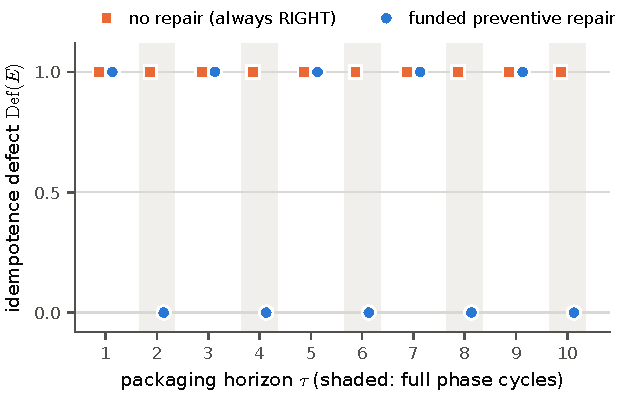
\includegraphics[width=0.72\linewidth]{figures/fig_packaging.pdf}
  \caption{Idempotence defect of the packaging map under the lens $(y,r,\phi)$, which hides the damage bit, in the funded ring world. Over the horizons shown, the defect is $1$ without repair, and with funded preventive repair it is $0$ at every full phase cycle (shaded) and $1$ at odd horizons, where the phase label necessarily changes. Markers are offset horizontally for visibility.}
  \label{fig:packaging}
\end{figure}

\begin{table}[t]
\centering
\small
\begin{tabular}{@{}lrr@{}}
\toprule
Regime (funded substrate) & $\mathrm{Def}(E)$ at $\tau=2$ & coherent $|\K|$ \\
\midrule
No repair: always move RIGHT & 1 & 0 \\
Funded preventive repair & 0 & 16 \\
Same policy, repair always fails & 0 & 0 \\
Idle without repair & 0 & 0 \\
\bottomrule
\end{tabular}

\caption{Packaging defect and coherent viability (safety $r\ge1$, $u=0$) in the funded ring world. ``Repair always fails'' keeps the funded repair policy but sets the repair success probability to $0$. ``Idle without repair'' replaces repair by a zero-cost action that does nothing. Both controls reach zero defect, but neither can keep any state coherent.}
\label{tab:packaging_controls}
\end{table}

\subsection{Controls: what zero defect does not show}
The repair policy reaches zero defect partly because it stops moving: an agent that stays in place keeps its position label. Two controls separate this effect from repair itself (\cref{tab:packaging_controls}). If the same policy is kept but repair always fails, the defect is still $0$; if the agent simply idles with no repair available, the defect is also $0$. In both cases the coherent viability kernel is empty: from every undamaged state the damage bit can flip with positive probability, and nothing resets it.

So in this system the contribution of repair is visible in viability, not in the packaging defect. The defect detects that coarse labels are self-reinforcing; viability detects that the hidden degrees of freedom are actually kept in order. The comparison is an existence witness under the named policies. It does not show that repair is necessary for low defect, and it does not show that zero modal defect implies stochastic persistence (\cref{sec:engine}).

\paragraph{Exact checks.}
The packaging maps were also computed with exact rational arithmetic and agree with the floating-point computation at $\tau=2$ for all four regimes. Some most-probable labels are exact ties, so the map depends on the tie-breaking rule. The separation does not: in the no-repair regime no admissible tie-break makes any label its own image, so every choice gives defect $1$; with funded repair every label in the image is the unique most probable label from itself, so every choice gives defect $0$.

\subsection{Interpretation}
In \SBT\ terms, a lens alone does not make an object. When hidden variables drift with nothing to compensate, the coarse labels either fail to be self-consistent or, if they are self-consistent, they hide a package that is quietly falling apart. Paid repair is a resource-accounting mechanism (P$_6$) that, together with closure (P$_5$), keeps the hidden variables in order; the viability kernel is the measure that registers it. The funded repair regime therefore supplies what the agent definition of \cref{sec:engine} requires on the agenthood side: a non-empty set of states that can be maintained, under a lens whose labels are object-like at the natural horizon.

\section{Null tests}
\label{sec:ex_nulls}

Empowerment measures difference-making, and precisely because it is a strong notion it can be produced by mistake. Two mistakes are common: confusing motion with control, and confusing outside structure with choice. Every later empowerment result should be read against the two null tests in this section.

\subsection{Null A: one action means no choice}
If only one action exists, there is only one action sequence, so the channel $W$ has a single row and its capacity is zero at every horizon. We check this on a three-state deterministic cycle with a single action. The system moves at every step, yet
\[
\Emp(H=1)=\Emp(H=2)=\Emp(H=3)=0 \text{ bits}.
\]
Being a moving subsystem is not the same as having agency; agency requires an input that can be set.

\subsection{Null B: the schedule trap}
Many systems contain an outside driver, such as a clock or schedule, that determines the next outside state. If this driver is wrongly treated as the agent's action, a control channel appears that does not exist.

Our minimal example has an outside state $x$ and a schedule bit $s_{\mathrm{ext}}$; at each step $x$ takes the value of $s_{\mathrm{ext}}$, and the schedule toggles. The agent has two actions, neither of which affects anything. In the \emph{correct} model the schedule is part of the state: starting with $x=0$ and the schedule bit equally likely to be $0$ or $1$, both actions produce the same distribution of $x$ after one step, so the channel rows are identical and the capacity is $0$. In the \emph{wrong} model the schedule is collapsed into the action, so ``choosing'' the action sets $x$ directly, and the capacity is $1$~bit (\cref{tab:nulls}).

\begin{table}[t]
\centering
\small
\begin{tabular}{@{}ll@{}}
\toprule
\textbf{Null test} & \textbf{Capacity (bits)} \\
\midrule
A: single action, $H=1,2,3$ & $0$, $0$, $0$ \\
B: schedule treated as an action (wrong model) & $1$ \\
B: schedule treated as state (correct model) & $0$ \\
\bottomrule
\end{tabular}
\caption{Null tests. A system without choice has zero empowerment at every horizon tested. An external schedule mistaken for an action produces a spurious bit, which disappears when the schedule is modelled as part of the state.}
\label{tab:nulls}
\end{table}

\subsection{Why the null tests matter}
The thesis that an agent is a theory object carries a modelling discipline: variables must be placed on the correct side of the interface. Null A stops us from calling every persistent moving pattern an agent. Null B stops us from crediting the agent with structure that belongs to its surroundings. In the experiments that follow, empowerment is computed only over actions that the ledger can pay for and that genuinely act on the ring-world state.

\section{Protocol cycles: when order matters}
\label{sec:ex_holonomy}

This experiment isolates P$_3$, the protocol cycle. If the effect of an interface move depends on \emph{when} it is made, then sequences of moves can reach outcomes that single moves cannot distinguish. The signature to look for is control that is equal at one step and larger over several steps.

\subsection{Setup}
We compare the reference ring world of \cref{tab:configs} with and without the protocol; the two configurations are otherwise identical. With the protocol on, LEFT and RIGHT move the agent one site at even phase and two sites at odd phase, so the effect of a move depends on the phase at which it is made. With the protocol off, every move is one site. In both regimes movement costs one unit, REPAIR is free, there is no income, the ledger holds at most two units, damage flips with probability $0.1$, and moves slip with probability $0.2$.

Safety is $r\ge1$. In both regimes the viability kernel contains all 64 states with $r\ge 1$, since the free REPAIR action leaves position and ledger unchanged. For each horizon $H=1,\dots,5$ we compute feasible empowerment to the position $y$, with all three actions as channel inputs and the initial-budget rule of \cref{sec:engine}, for the same 32 start states sampled from $\K$ (seed $0$), and report the median.

\subsection{Result: equal at one step, separated from two steps on}
\Cref{fig:protocol_horizon} shows the medians (in bits):
\begin{center}
\small
\begin{tabular}{@{}lccccc@{}}
\toprule
$H$ & 1 & 2 & 3 & 4 & 5 \\
\midrule
Protocol on  & 1.050 & 1.725 & 1.742 & 1.846 & 1.846 \\
Protocol off & 1.050 & 1.210 & 1.288 & 1.288 & 1.288 \\
\bottomrule
\end{tabular}
\end{center}
At $H=1$ the two regimes coincide. Here the reason can be checked directly: from any start state, the one-step channels of the two regimes differ only in whether the moved-to positions are one or two sites away, so they are the same channel up to a relabelling of outputs and have the same capacity. This is a property of these particular channels, not a general theorem about protocols. From $H=2$ on, the protocol regime has higher median empowerment, and the gap is largest (about $0.56$~bits) at $H=4$ and $5$. Neither curve can decrease with the horizon, because appending the free REPAIR action to every sequence leaves both the cost and the final position unchanged. Longer sequences can produce more distinguishable distributions of the final position, sometimes by reaching additional positions; the protocol curve gains more.

\begin{figure}[t]
  \centering
  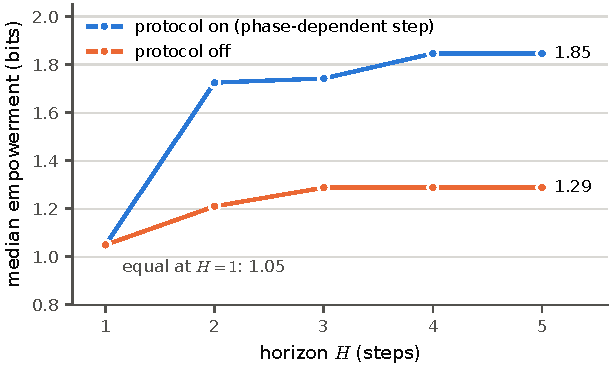
\includegraphics[width=0.72\linewidth]{figures/fig_protocol_horizon.pdf}
  \caption{Median feasible empowerment (bits) to the outside position $y$ as a function of horizon, with and without the phase-dependent step. Medians are over the same 32 start states sampled from the viability kernel. The curves coincide at $H=1$ and separate from $H=2$ on.}
  \label{fig:protocol_horizon}
\end{figure}

\subsection{A direct test of order dependence}
The medians aggregate many effects. For a sharper test we fix one start state, $s^\star=(y=0,\ u=0,\ \phi=1,\ r=2)$, and compare the two orders of the same moves, $\alpha=(\mathrm{RIGHT},\mathrm{LEFT})$ and $\beta=(\mathrm{LEFT},\mathrm{RIGHT})$. Both cost two units and are affordable from $r=2$. \Cref{tab:holonomy_witness} reports the total variation distance between the resulting distributions of $y$.

\begin{table}[t]
\centering
\small
\begin{tabular}{@{}lcc@{}}
\toprule
Damage noise & protocol on & protocol off \\
\midrule
$p_{\mathrm{flip}}=0.1$ (as in the exhibit) & 0.672 & 0.096 \\
$p_{\mathrm{flip}}=0$ (matched, noise-free damage) & 0.640 & 0.000 \\
\bottomrule
\end{tabular}

\caption{Total variation distance between the outside-position distributions produced by RIGHT-then-LEFT and LEFT-then-RIGHT from $s^\star=(y=0,u=0,\phi=1,r=2)$. Exact values: $84/125$ and $12/125$ with damage noise, $16/25$ and $0$ without it. The slip probability is $0.2$ in all four cases.}
\label{tab:holonomy_witness}
\end{table}

With the damage noise of the main experiment, order matters in both regimes ($0.672$ with the protocol, $0.096$ without). The second effect has nothing to do with the protocol: if damage occurs between the two moves, it reverses the direction of the second move, and the resulting displacement depends on which move came first. When damage noise is set to zero and everything else is kept, the protocol-free regime becomes exactly order-independent (distance $0$), while the protocol regime keeps a large order effect ($0.64$). This matched, noise-free pair isolates the protocol as the source of order dependence; the noisy pair shows that order effects in the full system also have other sources.

\subsection{Interpretation}
In \SBT\ terms, the protocol cycle is neither memory (P$_5$) nor budget (P$_6$): it concerns the order in which interface moves compose. In this substrate it leaves one-step control unchanged and enlarges multi-step control, without changing the viability kernel or the packaging lens. The agent's interface becomes more expressive over longer horizons; it can cause more distinguishable outcomes with the same moves and the same budget.

\section{Ablations}
\label{sec:ex_ablations}

The previous experiments isolated one mechanism at a time. Here we change single ingredients of the reference ring world, plus one combined change, and record all three measures, to see which measure responds to which change and where they can mislead.

\subsection{Measures}
Each row of \cref{tab:ablations} is a configuration that differs from the reference model (the protocol-on configuration of \cref{sec:ex_holonomy}) in the way named; all rows but one change a single ingredient, and the row ``free movement and REPAIR removed'' changes two. For each we report:
\begin{itemize}[leftmargin=*, itemsep=0.2em]
  \item $|\K|$, the size of the viability kernel for the safety predicate $r\ge1$ (staying funded; damage is not part of safety here);
  \item the median of $\Emp_{\mathrm{feas}}$ at $H=2$ to the position $y$, over 32 start states sampled from $\K$ with seed $0$, with all available actions as channel inputs;
  \item $\Def(E)$ at $\tau=2$ under the lens $(y,r,\phi)$ and a fixed reactive policy: REPAIR if damaged and affordable, otherwise RIGHT.
\end{itemize}

\begin{table}[t]
\centering
\small
\begin{tabular}{@{}lrrrr@{}}
\toprule
Configuration & States & $|\K|$ & Median $\Emp_{\mathrm{feas}}$ (bits) & $\mathrm{Def}(E)$ \\
\midrule
Reference model & 96 & 64 & 1.725 & 0.333 \\
\addlinespace
Protocol off (phase-independent step) & 96 & 64 & 1.210 & 0.333 \\
REPAIR action removed & 96 & 0 & 0.000 & 0.000 \\
Imperfect repair (success $0.5$) & 96 & 64 & 1.577 & 0.000 \\
Higher noise (flip $0.4$, slip $0.4$) & 96 & 64 & 1.208 & 0.333 \\
Free movement (move cost $0$) & 96 & 64 & 1.799 & 1.000 \\
Free movement and REPAIR removed & 96 & 64 & 0.807 & 1.000 \\
LEARN action added ($\theta\in\{0,1\}$) & 192 & 128 & 1.961 & 0.333 \\
\bottomrule
\end{tabular}

\caption{Ablations of the reference ring world (two phases with protocol, ledger $0$--$2$, movement cost $1$, free REPAIR, no income, $p_{\mathrm{flip}}=0.1$, $p_{\mathrm{slip}}=0.2$). ``States'' is the size of the state space. Median empowerment is at $H=2$ over 32 sampled viable states; $\Def(E)$ is at $\tau=2$ under the reactive policy described in the text. Adding LEARN doubles the state space and adds a channel input, so that row is not directly comparable with the others.}
\label{tab:ablations}
\end{table}

\subsection{Reading the table}
\paragraph{Viability responds to whether the ledger can be preserved.}
Removing REPAIR empties the viability kernel. The reason is specific to this configuration: there is no income, every move costs one unit, and the free REPAIR action is the only way to act without spending. Without it, every affordable action lowers the ledger, so no state can stay funded forever. This shows that viability detects the loss of a sustainable action; it is not, in this configuration, a statement about repairing damage, since damage plays no role in the safety predicate. (Damage-sensitive viability is studied in \cref{sec:ex_packaging,sec:ex_sweep}.) In every other row, including both free-movement rows, some action keeps the ledger at or above one, and $\K$ is the full set of states with $r\ge1$.

\paragraph{Empowerment responds to the protocol.}
The reference and protocol-off rows have the same viability kernel and the same defect, but median empowerment drops from $1.725$ to $1.210$~bits without the protocol, in line with \cref{sec:ex_holonomy}.

\paragraph{The cost ablation changes only costs.}
Setting movement costs to zero, with all actions kept, slightly raises median empowerment ($1.725$ to $1.799$~bits), since every two-step sequence becomes affordable. Removing costs \emph{and} REPAIR together gives $0.807$~bits. The large drop in that combined change therefore comes from losing the REPAIR action as a channel input, not from removing costs. With free movement the ledger can no longer run out and force the agent to stand still (the reactive policy still pauses to repair when damaged), and the defect is $1$.

\paragraph{The defect tracks whether the agent comes to rest.}
In this unfunded configuration the defect column mostly reflects ledger exhaustion rather than maintenance. In the rows without REPAIR and with imperfect repair, the most likely label two steps ahead always has an empty ledger; at $r=0$ the agent cannot pay to move and stays in place, so those labels are fixed points and the defect is $0$. In the reference model the agent pays to move while it can, and the labels that fail the idempotence test $E(E(x))=E(x)$ are exactly the 16 of 48 labels with a full ledger ($r=2$), giving a defect of $1/3$. The defect therefore cannot be read as a maintenance score across these rows. As in \cref{sec:ex_packaging}, a zero defect can come from coming to rest, and it is viability with an appropriate safety predicate that tracks maintenance.

\paragraph{Other perturbations.}
Higher noise lowers median empowerment to $1.208$~bits, and imperfect repair to $1.577$~bits, while $|\K|$ is unchanged because the safety predicate concerns only the ledger. These are quantitative perturbations of a single sampled median; changes in the state space can also change which states are sampled, so differences between rows should not be read as universal effect sizes.

\subsection{Summary}
\begin{itemize}[leftmargin=*, itemsep=0.25em]
  \item \textbf{Viability tracks sustainability.} Removing the only cost-free action, with no income, leaves no state that can be kept funded.
  \item \textbf{Protocol increases control.} With the same viability kernel, the phase-dependent step raises median empowerment at two steps.
  \item \textbf{Measures must be read for what they compute.} Removing costs alone barely changes empowerment, and a zero packaging defect can reflect an agent that has run out of resources and stopped.
\end{itemize}

\section{Noise and the cost of maintenance}
\label{sec:ex_sweep}

The packaging experiment showed that funded repair can keep a package coherent. Here we ask the complementary question: across levels of damage noise and repair cost, when can a coherent package be maintained at all?

\subsection{Setup}
We use the sweep configuration of \cref{tab:configs}: a single phase (no protocol), no slip, a ledger from $0$ to $7$, movement cost $1$, and an income of $4$ units whenever the agent lands on site $0$. Repair succeeds with certainty when executed. We vary the damage probability $p_{\mathrm{flip}}\in\{0,0.1,\dots,0.7\}$ and the repair cost from $0$ to $7$.

Safety requires both a funded ledger and no damage,
\[
\Safe = \{\, s : r(s)\ge 1 \ \text{and}\ u(s)=0 \,\},
\]
so the viability kernel contains the states that can be kept funded \emph{and} coherent with certainty under the model. At each grid point we compute $|\K|$ and the median of $\Emp_{\mathrm{feas}}$ at $H=2$ to the position $y$, over the first 16 states of $\K$ in index order (all of $\K$ when it has 16 states or fewer), with all three actions as channel inputs. When $\K$ is empty we report an empowerment of $0$ by convention.

\subsection{Result: a support change and a cost threshold}
\Cref{fig:sweep} shows both measures over the grid. Two features stand out.

\paragraph{All positive noise levels behave the same.}
Every tested positive damage probability gives the same viability kernel: $|\K| = 56, 7, 6, 5, 4$ for repair costs $0$ to $4$ and $|\K|=0$ from cost $5$ on. This is because viability depends only on which transitions are \emph{possible}, and any $p_{\mathrm{flip}}$ strictly between $0$ and $1$ makes the same transitions possible. The noise level matters only through the change from $p_{\mathrm{flip}}=0$ to $p_{\mathrm{flip}}>0$, which adds damage transitions. The boundary in the figure is therefore a change of support at zero noise combined with a cost threshold, not a gradual shrinking as noise grows.

\paragraph{Why the threshold sits at a repair cost of 4.}
When damage is possible, any action other than REPAIR can leave the agent damaged, so a coherent state can stay coherent with certainty only by repairing at every step. Repair does not move the agent, so its ledger changes each step by the local income minus the repair cost. Away from the income site this is negative whenever repair costs anything, so those states eventually run out. At the income site the income is $4$, so repair is sustainable exactly when it costs at most $4$, and it can be executed only from ledgers $r$ that cover its cost. For cost $c$ between $1$ and $4$ the kernel is the set of undamaged states at site $0$ with $c\le r\le 7$, which has $8-c$ elements; for $c=0$ every safe state can repair for free, giving all $8\times 7=56$ safe states. Without noise, coherence never breaks, the agent can keep itself funded by moving through the income site, and the kernel has between 46 and 56 states for every repair cost.

\begin{figure}[t]
  \centering
  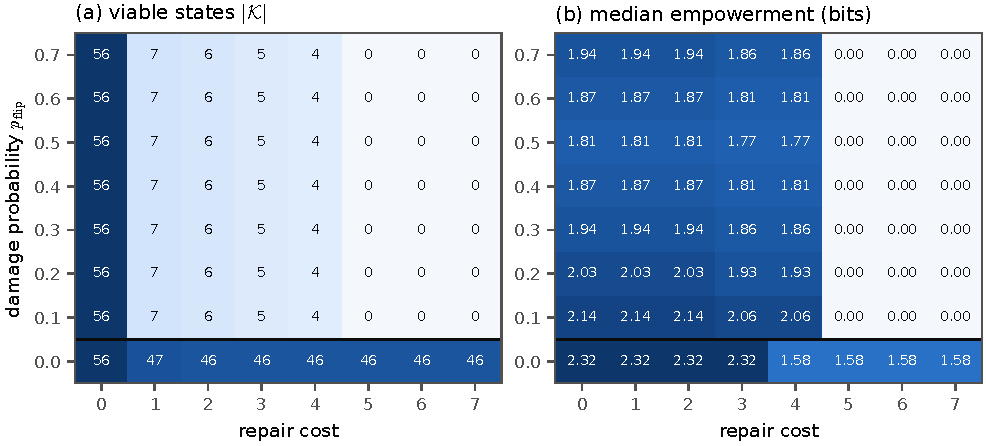
\includegraphics[width=\linewidth]{figures/fig_sweep.pdf}
  \caption{Noise--maintenance sweep with safety ``funded and undamaged''. \textbf{(a)} Size of the viability kernel. \textbf{(b)} Median feasible empowerment (bits) at $H=2$ over up to 16 viable start states; $0$ where the kernel is empty, by convention. The line separates zero noise from positive noise. Every positive noise level gives the same kernel; the kernel vanishes once repair costs more than the income of $4$ available at site $0$.}
  \label{fig:sweep}
\end{figure}

\paragraph{Empowerment.}
Without noise, median empowerment is $\log_2 5\approx 2.32$~bits for repair costs up to $3$ and $\log_2 3\approx1.58$~bits from cost $4$ on. With noise it lies between $1.77$ and $2.14$~bits wherever $\K$ is non-empty. On the grid it is smallest at $p_{\mathrm{flip}}=0.5$ and takes the same values at $p_{\mathrm{flip}}$ and $1-p_{\mathrm{flip}}$ (the pairs $0.3$/$0.7$ and $0.4$/$0.6$).

These positive values must be read with the scope of \cref{sec:engine} in mind. The channel inputs are open-loop sequences filtered only by the initial ledger, and most of them do not preserve coherence: when damage is possible, only REPAIR keeps the agent coherent with certainty, and a channel restricted to coherence-preserving moves would have zero capacity. The empowerment panel therefore measures how much an agent that \emph{starts} in a maintainable state can influence its position, not how much it can influence it while staying coherent. The two panels coincide in where empowerment is zero only because empty kernels are reported as zero.

\subsection{Interpretation}
This is the clearest instance in the paper of maintenance as a condition for agenthood under noise. Resource accounting (P$_6$) provides the means of paying for coherence, feasibility (P$_2$) decides whether that payment can actually be made, and closure (P$_5$) turns the two into an invariant set. When the income available at a sustainable location can no longer cover the cost of repair, the maintained package disappears, $\K=\emptyset$, and with it the domain on which the agent's actions were defined.

\section{Skill as a change of law}
\label{sec:ex_learning}

This experiment isolates P$_1$, operator rewriting. In \SBT, learning in this sense is not storing facts but changing the effective transition law, so that the same interface moves become more reliable. If that is right, higher skill should show up as more difference-making under the same constraints.

\subsection{Setup}
We use the skill configuration of \cref{tab:configs}. A skill level $\theta\in\{0,1,2\}$ is part of the state and lowers the slip probability from $0.40$ to $0.25$ to $0.10$. A LEARN action raises $\theta$, but it is not used as a channel input here: we compare fixed skill levels rather than modelling a learning process. There is no protocol, no damage noise, and no repair, and all actions are free, so every sequence is affordable and $\Emp_{\mathrm{feas}}=\Emp$.

The skill level indexes sectors of the kernel with different slip, so changing $\theta$ changes the transition law that the agent's moves obey, rather than adding a record that the agent consults. For each $\theta$ we compute empowerment at $H=2$ to the position $y$, with LEFT and RIGHT as channel inputs, from every undamaged state of the viability kernel (safety $r\ge1$) with that skill level, and report the median.

\subsection{Result}
Median empowerment rises with skill (\cref{fig:learning_theta}):
\[
0.841 \ (\theta=0), \qquad 1.052 \ (\theta=1), \qquad 1.370 \ (\theta=2) \ \text{bits}.
\]
With less slip, the same two-move sequences produce more sharply separated distributions of the outside position, so more of them can be told apart from the outcome.

\begin{figure}[t]
  \centering
  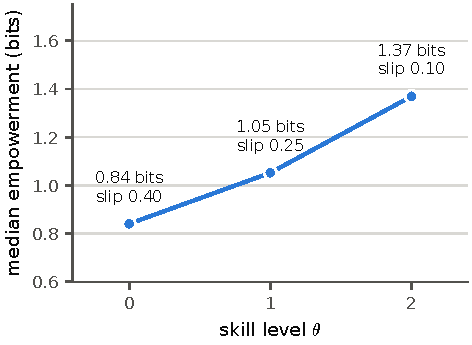
\includegraphics[width=0.5\linewidth]{figures/fig_learning_theta.pdf}
  \caption{Median empowerment (bits) at $H=2$ to the outside position, by skill level. Each skill level lowers the slip probability, shown under each value; medians are over all undamaged viable states at that level.}
  \label{fig:learning_theta}
\end{figure}

\subsection{Interpretation}
Packaging and viability (P$_5$, P$_6$) make a package persist, and protocol cycles (P$_3$) add reach over longer horizons. Operator rewriting acts on something else: the effective law of the induced level. Raising $\theta$ makes interface moves map to outside consequences more reliably, so the agent can make more distinguishable differences with the same moves. In the language of the thesis, the theory is unchanged as a level of description, but the theory object it hosts becomes a better channel from interface to outside. The experiment is stylised: skill is a fixed parameter that scales one noise source, and we do not model how it is acquired.

\section{Reproducibility and verification}
\label{sec:repro}

Every number in this paper is produced by deterministic scripts from hashed configurations, and every step from code to manuscript can be rerun and checked. This section lists what is checked, how, and what each check does and does not establish.

\subsection{Artefacts}
Experiment outputs are written under \texttt{results/}. Each JSON artefact records its configuration, a stable hash of that configuration (also used in file names), the measured quantities, a creation time, and library versions. The ablation artefacts also record the sampled start states and the per-state capacities behind each median, and the sweep records its sampling rule; the protocol and skill artefacts record the medians, whose constituent values can be recomputed from the stored configurations. The strict auditor checks that required fields are present, that every stored hash matches its configuration, that probability objects are valid, and that sweep arrays and packaging defects are well formed. It validates structure and consistency; it does not certify scientific claims.

A single export script produces the manuscript's data figures and generated tables. The figures and the ablation table are read from the artefacts above; the packaging-control table and the order-witness table are computed by the export script directly from the stated configurations. The script also writes the cited scalars and their configuration hashes to \texttt{paper/generated/numbers.json}. The configuration and dictionary tables are part of the manuscript source. Sampling uses a fixed seed and recorded rules (\cref{tab:configs}).

\subsection{Independent checks}
Three further layers check the mathematics rather than the bookkeeping.
\begin{itemize}[leftmargin=*, itemsep=0.25em]
  \item \textbf{Tests.} The test suite (80 tests) includes channels with known capacity, such as a Z-channel with capacity $\log_2(5/4)$, channels with redundant rows, failure on non-convergence, and an exhaustive comparison of the viability computation against a brute-force search over all $5{,}184$ systems with two states and two actions (all non-empty supports, feasible-action sets, and safe sets). It also retains the two-state counterexample of \cref{sec:engine}.
  \item \textbf{Exact arithmetic.} A review script recomputes, with exact rational arithmetic and at $\tau=2$, the packaging maps of the funded comparison and of the failed-repair control of \cref{sec:ex_packaging}, together with an idle control in the unfunded variant of the substrate (which also has zero defect and an empty coherent kernel), and the order witnesses of \cref{sec:ex_holonomy}. It compares each relevant floating-point transition row with its exact counterpart and checks the tie-breaking conditions of the packaging separation.
  \item \textbf{Lean.} The finite fixed-point and viability results of \cref{sec:engine} are proved in Lean~4 with mathlib \citep{demoura2021lean4,mathlib2019} (\cref{app:lean_viability}). An audit file prints the axioms each exported theorem depends on: only Lean's standard \texttt{propext}, \texttt{Classical.choice}, and \texttt{Quot.sound}. There are no unproved steps, custom axioms, or calls to \texttt{native\_decide}.
\end{itemize}
The Lean results concern the abstract operator on finite sets. The step from the Python code, which reads supports off floating-point kernels, to those finite sets is tested but not mechanised; channel capacities and packaging maps are not formalised in Lean.

\subsection{Commands}
From the repository root:
\begin{verbatim}
pip install -e '.[dev]'
pytest -q
(cd lean && lake build && lake env lean Audit.lean)
python scripts/review_mathematics.py
python scripts/run_all_experiments.py --clean
python scripts/audit_results.py --strict
python scripts/export_paper_assets.py --no-run
python scripts/build_paper.py
\end{verbatim}
The experiment runner regenerates the experiment artefacts and ends with the strict audit; the export script then generates the manuscript's figures and tables. The null tests of \cref{sec:ex_nulls} are standalone scripts (\texttt{scripts/null\_single\_action.py} and \texttt{scripts/null\_schedule\_trap.py}) and are also covered by the test suite.

\section{Discussion: an agent is a theory object}
\label{sec:discussion}

\paragraph{The thesis, restated.}
In \SBT\ \citep{six_birds_theory}, a theory is an induced level of description; in this paper it is the finite specialisation $T=(\Pi,L,\mathcal{F},B)$. An agent is not that level. It is a \emph{theory object}: a maintained package inside the level, with a ledger-gated interface whose settings make a difference to outside futures within the induced dynamics. Agenthood is the existence and maintenance of the package; agency is the causal reach of its interface. Rather than adding agency as an extra ingredient, the framework asks which mechanisms must be in place for ``throwing a stone'', stable counterfactual difference-making under constraints, to become a meaningful statement at an induced scale.

\subsection{Enablement and causation}
The distinction between agenthood and agency is the distinction between enablement and causation.

Enablement is about making variables and objects exist stably. Packaging produces coarse labels and an interface; accounting produces a ledger that can be earned and spent; constraints turn commands into actions; staging fixes the horizons on which labels can stabilise. In our setting, the viability kernel is the sharpest measure of enablement: if $\K=\emptyset$, nothing can be maintained with certainty, and there is no stable package whose choices one could discuss.

Causation is about difference-making once the variables exist: within a fixed level, does changing the actions change the distribution of the outside variable $H$ steps later? Feasible empowerment measures this for open-loop, budgeted action sequences. The schedule trap shows why the two must be kept apart: importing an enablement mistake (treating outside structure as an action) into the causal level fabricates agency.

The experiments separate the two axes in both directions. A phase-dependent step raises empowerment without changing the viability kernel (\cref{sec:ex_holonomy}). Funded repair creates a coherent viability kernel, while the packaging defect cannot distinguish it from an agent that merely stops moving (\cref{sec:ex_packaging}). And under damage noise, open-loop empowerment from viable states is positive even though only repair preserves coherence (\cref{sec:ex_sweep}).

\subsection{Relation to life}
The companion paper on life \citep{six_birds_life} treats life as closure and maintenance: a package that persists by paying for its own repair. The present paper adds an ingredient that life as such does not require, namely an interface whose choices reach the outside in a stable way. Life leans on closure (P$_5$) and accounting (P$_6$); agency adds a genuine action channel, which protocol cycles (P$_3$) can widen and operator rewriting (P$_1$) can sharpen. This matches ordinary intuition: many living systems persist with little horizon-dependent control, and many controlled devices act without maintaining themselves.

\subsection{Limitations}
\paragraph{Small, exact systems.}
The ring worlds in the reported experiments have at most 192 states. This makes every computation exact or numerically converged and fully auditable, but the results are finite existence witnesses under named configurations and policies. The definitions do not depend on scale; the evidence does.

\paragraph{Open-loop, initial-budget empowerment.}
Feasible empowerment uses action sequences fixed in advance and filtered by the initial ledger. It does not check affordability step by step when the ledger changes along the way, and it does not require the sequences to stay viable or safe. A positive value from a viable state is therefore not a capacity of safe behaviour. Closed-loop and safety-constrained versions are natural refinements.

\paragraph{Modal objecthood.}
The packaging defect is a property of a most-probable-label map that restarts from a uniform fibre. Zero defect does not imply that the coarse labels form an autonomous stochastic process, and it can arise from an agent that has simply stopped. We use it together with viability, not as a stand-alone measure of objecthood.

\paragraph{Lens and policy dependence.}
Empowerment depends on the output lens, packaging on the macro lens and the maintenance policy, and viability on the safety predicate. In \SBT\ these choices are part of specifying the level of description. Our comparisons use stated lenses, safety predicates, and policies, and where a comparison changes the policy, as in the packaging controls, the change is explicit; every statement is relative to these choices.

\paragraph{Support semantics.}
Viability asks that every possible successor be safe. This suits robust closure claims but is strict: as the sweep shows, any positive noise, however small, changes the result. Risk-sensitive or probabilistic variants would change the safe set and the operator but keep the fixed-point structure.

\paragraph{Uneven coverage of the mechanisms.}
Protocol cycles and paid maintenance are tested by matched comparisons. Operator rewriting is represented by fixed skill levels rather than a learning process. Identity is not exercised at all, and staging only through the phase. Sampled medians depend on the sampling rule, and capacities are floating-point approximations with numerical, not certified, error bounds.

\paragraph{What is assumed.}
The interface (which variables are actions) is given, not discovered from microdynamics; discovering it is itself a packaging problem. The ledger is an abstract resource, not a thermodynamic quantity. We model a single agent, with no social interaction or norms.

\paragraph{What we do not claim.}
We do not claim that agency requires consciousness, that empowerment is the measure of agency, that a ring world captures real organisms, or that agents must have goals or utilities. Nor do we claim that repair is necessary for objecthood, or that the Lean proofs cover the stochastic or information-theoretic parts of the pipeline. The claim is narrower: once an induced level maintains a package under budgets, agency can be read as the existence of a genuine, correctly typed action channel that makes stable counterfactual differences at the relevant horizon, and each part of that reading can be computed and checked.

\subsection{Outlook}
Three directions follow. First, multi-agent settings, in which constraints (P$_2$) and identity tokens (P$_4$) can express commitments, ownership, and norms. Second, learned approximate models in place of exact kernels, keeping the same audit discipline. Third, alternative causal measures, such as closed-loop or safety-constrained empowerment, reachable-set volumes, and interventional effect sizes, and a study of when they agree.

\paragraph{Conclusion.}
To throw a stone is to have an interface whose choices reach the outside in a stable way under constraints. The six birds explain how that statement can become true: closure and accounting let a package persist, constraints decide which actions exist, and protocol cycles and operator rewriting extend what those actions can do. In this sense an agent is a theory object: not the level of description itself and not an inner narrative, but a maintained object of that level whose interface variables become causes in the induced dynamics.

\section*{Declarations}

\paragraph{Corresponding author.}
Correspondence to Ioannis Tsiokos (\texttt{ioannis@automorph.io}).

\paragraph{Competing interests.}
The author declares no competing interests.

\paragraph{Funding.}
No external funding was received for this research.

\paragraph{Ethics approval and consent to participate.}
Not applicable; this study involves computational experiments only and uses no human participants, animal subjects, or personal data.

\paragraph{Data availability.}
All generated artefacts (JSON, CSV, and NPZ files) are produced by the included scripts and are available in the repository and the archived release. No external datasets were used.

\paragraph{Code availability.}
Source code is available at \url{https://github.com/ioannist/six-birds-agent}. A permanent archive of the code is deposited at Zenodo under DOI \href{https://doi.org/10.5281/zenodo.18451887}{10.5281/zenodo.18451887}.

\paragraph{Author contributions.}
I.T.\ is the sole author and was responsible for conceptualisation, methodology, software, formal analysis, writing, and visualisation.

\paragraph{Use of AI/LLMs.}
LLM tools (Claude, Anthropic; Codex, OpenAI) were used as coding assistants, for mathematical review of the code and proofs, and for editing and checking the manuscript text. The author designed the study, reviewed and validated all outputs, and takes responsibility for the content.


\appendix
\section{The Lean development}
\label{app:lean_viability}

The file \texttt{lean/Agency/Viability.lean} formalises the finite fixed-point argument behind the viability computation of \cref{sec:engine}, in Lean~4 with mathlib \citep{demoura2021lean4,mathlib2019}. This appendix states its results in mathematical form; Lean names are given in parentheses.

\paragraph{Bounded stabilisation from any finite start.}
Let $F$ be a map on finite subsets of a type $\alpha$ that is contracting, $F(K)\subseteq K$ for all $K$, and let $K_0$ be a finite set. Then some iterate $F^n(K_0)$ with $n\le |K_0|$ is a fixed point (\lean{iterate_stabilizes_bounded}). The bound counts strict removals: each iteration that changes the set removes at least one element. No finiteness of $\alpha$ and no decidable equality on it are assumed. If $F$ is also monotone, this fixed point contains every fixed point $S\subseteq K_0$ (\lean{iterate_greatest_fixpoint_bounded_from}).

\paragraph{The viability operator.}
For a safe set $\Safe$, feasible-action sets $\Afeas(s)$, and successor sets $\Post(s,a)$, the operator
\[
\mathcal{V}(K)=\{s\in K : s\in\Safe \text{ and } \exists a\in\Afeas(s),\ \Post(s,a)\subseteq K\}
\]
is proved to be contracting and monotone (\lean{viabilityOperator_contracting}, \lean{viabilityOperator_monotone}); these are theorems about the operator, not hypotheses. Its fixed points are exactly the sets $K\subseteq\Safe$ in which every state has a feasible action with $\Post(s,a)\subseteq K$ (\lean{viabilityOperator_fixpoint_iff}).

\paragraph{The kernel computed from the safe set.}
Iterating $\mathcal{V}$ from $\Safe$, as the implementation does, reaches after $n\le|\Safe|$ steps a safe controlled-invariant set that contains every safe controlled-invariant set (\lean{viability_iteration_greatest_bounded}). This is the viability kernel. In the implementation, whose recorded history includes the starting set and the final repeated set, this means at most $|\Safe|+1$ evaluations of the operator.

\paragraph{Feedback and pathwise safety.}
Controlled invariance of $K$ yields a stationary selector that assigns to each state of $K$ a feasible action whose successor set lies in $K$; it is defined only on $K$, so an empty $K$ needs no default action (\lean{controlledInvariant_stationary_policy}). For any policy with $\Post(s,\mathrm{policy}(s))\subseteq K$ on $K$, every path that starts in $K$ and whose steps stay within the successor sets remains in $K$ forever (\lean{stationary_policy_paths_safe}). This is pathwise safety; it involves no probabilities.

\paragraph{The top-set form.}
The development also exports the classical form (\lean{iterate_top_greatest_fixpoint}): for monotone, contracting $F$ on the finite subsets of a finite type, some iterate of $F$ from the full set is a fixed point containing every fixed point. A strengthened form adds the bound $n\le|\alpha|$ (\lean{iterate_top_greatest_fixpoint_bounded}).

\paragraph{Scope.}
The general operator allows empty successor sets, so its invariance results hold in that generality; interpreting them as statements about a stochastic process requires non-empty supports, which the Python code enforces. The correspondence between the floating-point kernels and these finite sets is tested, not proved. Probabilities, channel capacities, and packaging maps are outside the formalisation. The audit file \texttt{lean/Audit.lean} prints the axioms used by each exported theorem: \texttt{propext}, \texttt{Classical.choice}, and \texttt{Quot.sound}, with the pathwise-safety theorem using only \texttt{propext} and \texttt{Quot.sound}.

\section{Version history}
\label{app:versions}

\paragraph{Version 1 (31 January 2026).}
First public version (Zenodo, DOI \href{https://doi.org/10.5281/zenodo.18439737}{10.5281/zenodo.18439737}).

\paragraph{Version 2.}
Editorial and formatting changes in preparation for preprint-server submission; no change to results.

\paragraph{Version 3 (6 October 2026).}
A review of the mathematics and code led to the following changes.
\begin{itemize}[leftmargin=*, itemsep=0.2em]
  \item The capacity computation now uses the standard Blahut--Arimoto update, including the factor $p_k(\alpha)$, and stops on an explicit gap between lower and upper bounds. All empowerment values were recomputed. The protocol and skill separations survive the correction; the cost-only and combined cost-and-repair ablations are now distinguished.
  \item The packaging experiment now uses a funded substrate in which every repair is affordable and can be sustained. The previous setup could not pay for sustained repair, and part of its policy issued unaffordable commands. Controls were added showing that a zero packaging defect does not by itself indicate maintenance.
  \item The order-dependence witness is reported both with damage noise, where the protocol-free regime also shows order effects, and in a matched noise-free form.
  \item The cost ablation now changes only movement costs; the earlier combined change, which also removed repair, is reported separately. The identity setting now affects the state space when switched off, although the reported ring-world experiments use a single identity value.
  \item The noise--maintenance sweep is explained as a change of support at zero noise plus a repair-cost threshold.
  \item The scope of feasible empowerment (open-loop, initial budget, not restricted to safe behaviour) and the modal character of the packaging defect are stated explicitly.
  \item The Lean development was extended to the viability operator itself, with a bound on the number of iterations, a characterisation of fixed points, and pathwise safety of invariant feedback.
  \item The exposition, figures, and tables were revised throughout.
\end{itemize}

\clearpage
\bibliographystyle{plainnat}
\bibliography{bib/refs}
\end{document}
